\documentclass{uebblatt}

\begin{document}

\maketitle{8}{}
\enlargethispage{1em}

\begin{aufgabe}{Was tun, wenn das terminale Objekt nicht kofasernd ist?}
\emph{Diese Aufgabe ist offen gestellt und soll zum Experimentieren einladen.}
Bekanntlich gibt es folgende Aussage (Lemma~16.4.9 in May/Ponto): Sei~$\V$ eine
kartesisch abgeschlossene monoidale Modellkategorie. Sei das terminale
Objekt~$\star$ kofasernd. Dann wird die Modellkategorie~$\V_\star$ der punktierten
Objekte mit dem Smash-Produkt zu einer monoidalen Modellkategorie.

Sei in diesem Kontext das terminale Objekt nicht kofasernd. Welche Bedingung könnte man
stellen, damit~$QS^0 \wedge X \to S^0 \wedge X$ immer noch für alle kofasernden
Objekte~$X$ eine schwache Äquivalenz ist? Dabei ist~$S^0$ das Einsobjekt
von~$\V_\star$.
\end{aufgabe}

\begin{aufgabe}{Euler-Charakteristik in symmetrisch monoidalen Kategorien}
Ein Objekt~$X$ einer symmetrisch monoidalen Kategorie heißt genau dann
\emph{dualisierbar}, wenn es ein Objekt~$X^\vee$ zusammen mit Morphismen~$I
\xra{\eta} X \otimes X^\vee$ und~$X^\vee \otimes X \xra{\varepsilon} I$ gibt,
welche die Dreiecksidentitäten erfüllen:
\[ (\id_X \otimes \varepsilon) \circ (\eta \otimes \id_X) = \id_X \qquad
  (\varepsilon \otimes \id_{X^\vee}) \circ (\id_{X^\vee} \otimes \eta) = \id_{X^\vee}. \]
Die \emph{Spur} eines Endomorphismus~$f : X \to X$ eines dualisierbaren
Objekts~$X$ ist die Verkettung~$I \stackrel{\eta}{\lra} X \otimes X^\vee
\stackrel{f \otimes \id}{\lra} X \otimes X^\vee \lra X^\vee \otimes X
\stackrel{\varepsilon}{\to} I$.
\begin{enumerate}
\item Was ist nach dieser Definition die Spur eines Endomorphismus eines
endlich-dimensionalen~$k$-Vektorraums?
\item Zeige allgemein: Die Spur von~$f \circ g$ ist gleich der Spur von~$g
\circ f$.
\item Die Kategorie~$\mathrm{Cob}_n$ hat als Objekte
geschlossene~$(n-1)$-Mannigfaltigkeiten. Morphismen~$M \to N$
sind Diffeomorphieklassen von~$n$-Mannigfaltigkeiten~$W$ mit~$\partial W = M
\amalg N$. Wie sollte man die Verknüpfung definieren? Wie eine symmetrisch
monoidale Struktur, in der das Tensorprodukt durch disjunkte Vereinigung
gegeben ist? Wieso ist bezüglich dieser jedes Objekt dualisierbar? Was
ist die Spur eines Endomorphismus in dieser Kategorie?
\end{enumerate}
\end{aufgabe}

\begin{aufgabe}{Präzise Definitionen}
\begin{enumerate}
\item Buchstabiere die Definitionen von monoidalen Funktoren und (Rechts-)Moduln über
monoidalen Kategorien aus.
\item Sei~$F : \C \to \D$ ein monoidaler Funktor. Wie
wird~$\D$ zu einem~$\C$-Modul?
\end{enumerate}
\end{aufgabe}

\centering
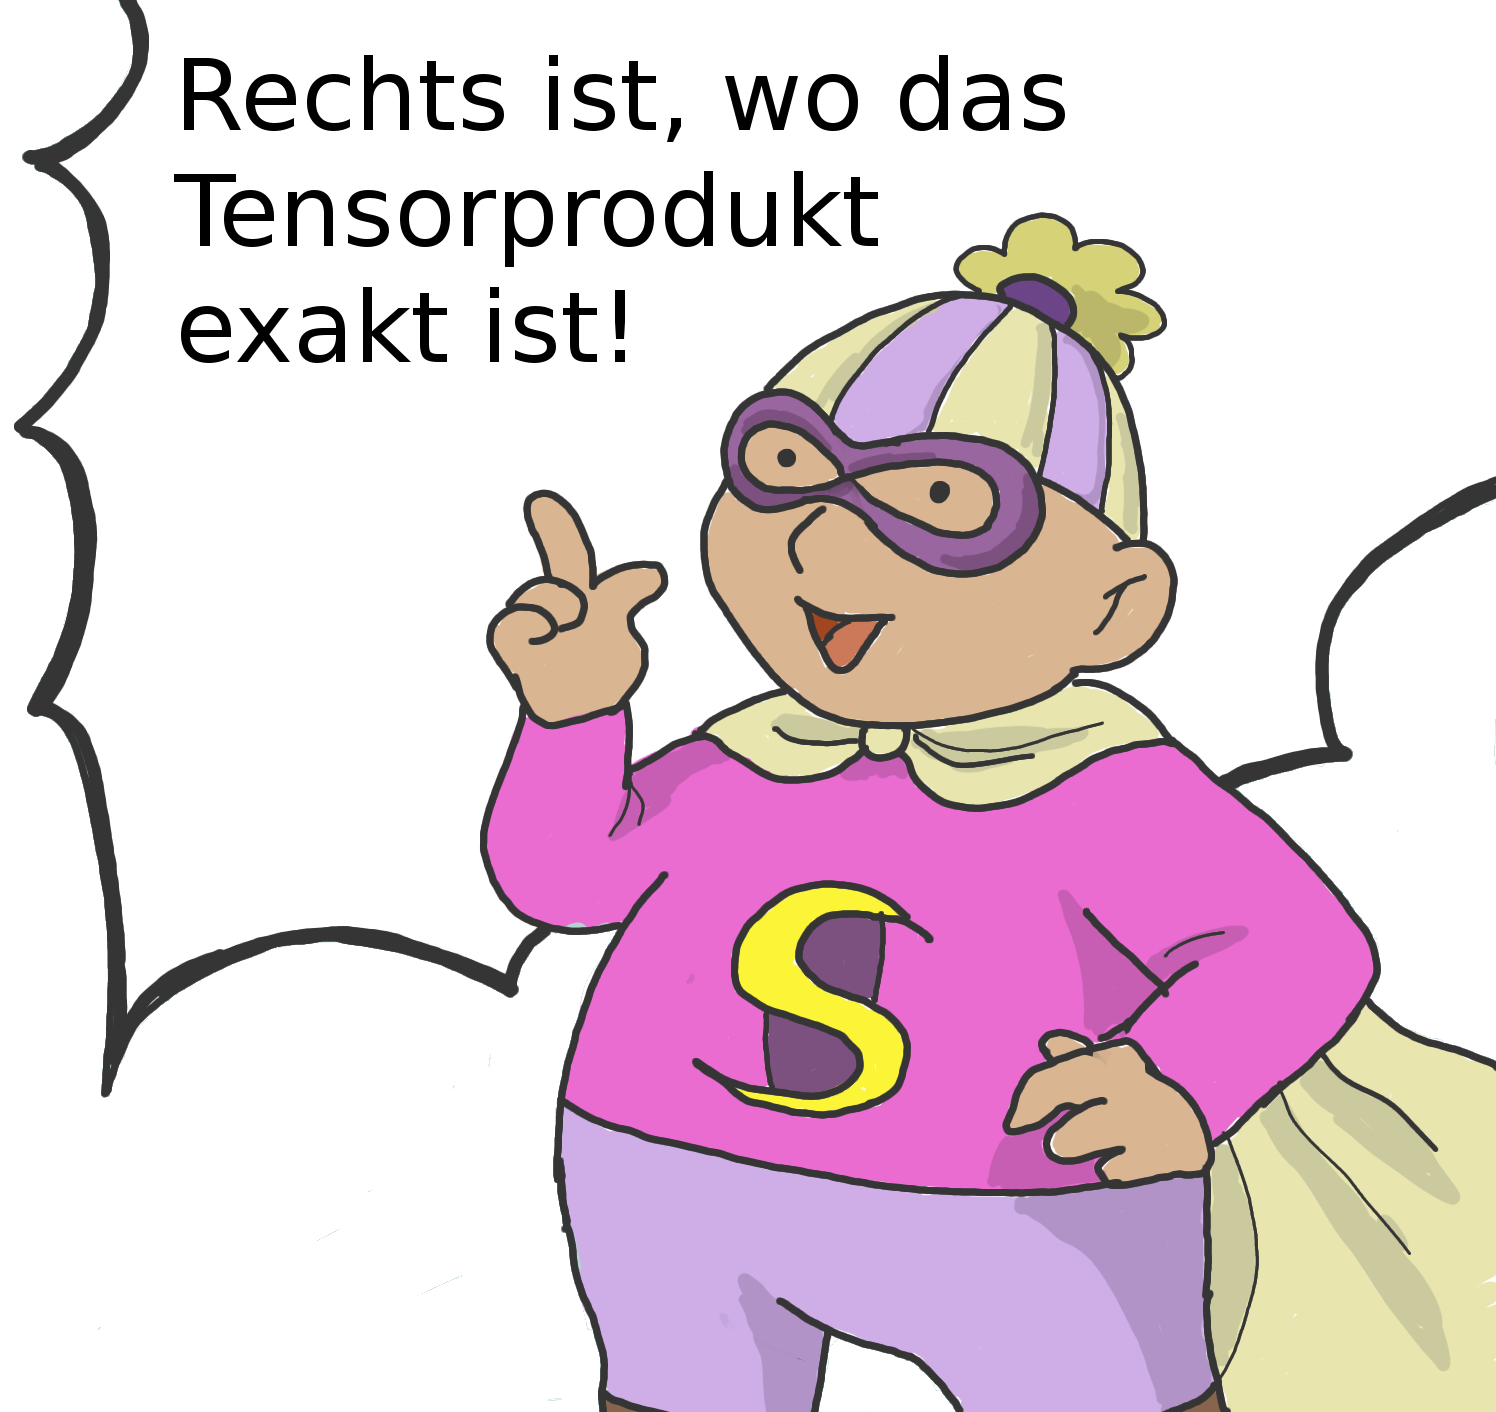
\includegraphics[scale=0.08]{images/rechts-ist-wo-das-tensorprodukt-exakt-ist}
\par

\end{document}
